\documentclass[cic,tc,english]{iiufrgs}

\usepackage[utf8]{inputenc}
\usepackage{graphicx}
\usepackage{times}
% \usepackage{palatino}
% \usepackage{mathptmx}       % p/ usar fonte Adobe Times nas fórmulas

\usepackage[alf,abnt-emphasize=bf]{abntex2cite}

\usepackage{lipsum}

\usepackage{revisornotes}
\usepackage{draftenvironment}

\usepackage{ragged2e}

\usepackage{listings}

\usepackage{amsmath}      % For math symbols
\usepackage[boxed]{algorithm}    % For the algorithm environment
\usepackage{algpseudocode} % For pseudocode formatting
\usepackage{xcolor}       % Optional for colored comments
\usepackage{caption}      % For captions in algorithms

\usepackage{tikz}

\usepackage{amsfonts}

\usepackage[bottom]{footmisc}

\usepackage{amssymb}

\numberwithin{algorithm}{chapter}

\title{
    A Hybrid Multi-Authority Attribute-Based Encryption Scheme For Securing hIoT Data
}
\translatedtitle{
    Um Esquema Híbrido de Criptografia Baseada em Atributos de Múltiplas Autoridades para Armazenamento Segura de Dados hIoT
}

\author{Graeff}{Felipe de Almeida}

\advisor[Prof.~Dr.]{Nobre}{Jéferson Campos}
\coadvisor[M.Sc]{Soares}{Laura Rodrigues}

% \date{maio}{2001}
% \location{Itaquaquecetuba}{SP}

\keyword{MA-ABE}
\keyword{hybrid cryptography}
\keyword{access control}
\keyword{HIoT}
\keyword{data security}
\keyword{performance analysis}
\keyword{decentralized systems}

\translatedkeyword{MA-ABE}
\translatedkeyword{criptografia híbrida}
\translatedkeyword{controle de acesso}
\translatedkeyword{HIoT}
\translatedkeyword{segurança de dados}
\translatedkeyword{análise de desempenho}
\translatedkeyword{sistemas descentralizados}

%\settowidth{\seclen}{1.10~}

\begin{document}

\maketitle

% dedicatory
\clearpage
\begin{flushright}
    \mbox{}\vfill
    \begin{tabular}{p{0.55\linewidth} p{0.45\linewidth}}
        In loving memory of Professor Raul Fernando Weber, a remarkable educator and influential figure in the field of computer security. His passion for teaching and dedication to his students left an indelible mark on all who had the privilege to learn from him. As I embark on my undergraduate thesis in computer security, I humbly dedicate this work to the memory of a great professor and a charismatic person who inspired generations of students, including myself. His guidance and enthusiasm ignited my love for this area, and I am forever grateful for the knowledge and inspiration he shared. His legacy lives on in the pursuit of knowledge and excellence. Rest in peace, \mbox{Professor} Weber.\\
    \end{tabular}
\end{flushright}

\chapter*{Acknowledgements}
    I would like to express my sincere gratitude to my advisor, Professor Jéferson Campos Nobre. I am thankful for his trust and for providing me with the opportunity to develop this research in a field I am passionate about. His efforts and his knowledge in the computer security area that he brought to UFRGS have created a vital and inspiring environment for students, and I am grateful for the academic freedom and encouragement he provided throughout this journey.

    I also extend my deepest gratitude to my co-advisor, Laura Rodrigues Soares. Her foundational research laid the groundwork for this thesis, and her constant guidance, dedication, and hands-on support were a driving force behind this project. Her collaboration was essential to its success from start to finish.

    My appreciation also extends to the faculty and staff at the Informatics Institute. The education and support provided by the professors have been fundamental to my academic and professional growth. Their dedication to creating a nurturing and challenging academic environment has been critical to my development.

    Special thanks go to Valéria, my best friend, for her constant support and love. Her encouragement has been a pillar of strength in difficult times, reminding me of the value of perseverance.

    I am grateful to all my friends for their continued encouragement and belief in my abilities. Their support and the occasional much-needed distractions have helped me maintain my focus and passion for my research.

    Finally, I would like to thank Marina and Pedro, my psychologist and psychiatrist. Their professional support has been crucial in managing the stress of my academic commitments, significantly contributing to my well-being and success.

    This thesis reflects the collective support and encouragement of all those mentioned and many others, to whom I am deeply thankful.

\clearpage
\begin{flushright}
    \mbox{}\vfill
    \begin{minipage}{0.49\textwidth}
        % \setlength{\baselineskip}{1.2em} % Adjust line spacing
        \justifying
        \noindent
        {\itshape
        ``That is what I have always understood to
        be the essence of anarchism: the conviction
        that the burden of proof has to be placed on 
        authority, and that it should be dismantled 
        if that burden cannot be met.''\\
        }
        
        \raggedleft
        \parbox{\linewidth}{--- \textsc{Noam Chomsky,} \textit{Red and Black Revolution, No. 2} (May 1995)}
    \end{minipage}
\end{flushright}


\begin{abstract}
    The proliferation of Health Internet of Things (HIoT) devices has created an urgent need for secure and decentralized data sharing mechanisms that protect sensitive patient information while enabling flexible access for multiple stakeholders. Existing decentralized storage architectures for HIoT often lack a concrete cryptographic layer that provides fine-grained access control, leaving data vulnerable to unauthorized access. This thesis addresses this gap by proposing, implementing, and evaluating a hybrid cryptographic scheme that combines Multi-Authority Attribute-Based Encryption (MA-ABE) with symmetric Advanced Encryption Standard (AES) encryption to secure HIoT data. The proposed solution leverages the MaabeRW15 scheme to allow access policies to be defined over attributes distributed across multiple independent authorities, while efficient AES encryption is used for large data payloads. A comprehensive performance evaluation of a proof-of-concept implementation was conducted to measure the system's scalability and computational overhead. The results demonstrate that the hybrid approach is efficient for securing large datasets and that system performance scales effectively with process-based concurrency, though it is sensitive to the complexity of access policies and high user loads. This work confirms the viability of the proposed scheme as a practical method for enforcing robust, fine-grained access control in decentralized HIoT data management systems, offering a significant enhancement to data privacy and security.
\end{abstract}

\begin{translatedabstract}
    A proliferação de dispositivos de Internet das Coisas para Saúde (HIoT) gerou uma necessidade urgente de mecanismos seguros e descentralizados para o compartilhamento de dados, que protejam as informações sensíveis dos pacientes e, ao mesmo tempo, permitam o acesso flexível por múltiplas partes interessadas. As arquiteturas de armazenamento descentralizado existentes para HIoT frequentemente carecem de uma camada criptográfica concreta que forneça controle de acesso de granularidade fina, deixando os dados vulneráveis a acessos não autorizados. Esta tese aborda essa lacuna ao propor, implementar e avaliar um esquema criptográfico híbrido que combina Criptografia Baseada em Atributos de Múltiplas Autoridades (MA-ABE) com a criptografia simétrica Advanced Encryption Standard (AES) para proteger dados de HIoT. A solução proposta utiliza o esquema MaabeRW15 para permitir que políticas de acesso sejam definidas sobre atributos distribuídos entre múltiplas autoridades independentes, enquanto a criptografia AES é usada de forma eficiente para grandes volumes de dados. Uma avaliação de desempenho abrangente de uma prova de conceito foi conduzida para medir a escalabilidade e o custo computacional do sistema. Os resultados demonstram que a abordagem híbrida é eficiente para proteger grandes conjuntos de dados e que o desempenho do sistema escala efetivamente com a concorrência baseada em processos, embora seja sensível à complexidade das políticas de acesso e a altas cargas de usuários. Este trabalho confirma a viabilidade do esquema proposto como um método prático para impor um controle de acesso robusto e de granularidade fina em sistemas descentralizados de gerenciamento de dados de HIoT, oferecendo uma melhoria significativa na privacidade e segurança dos dados.
\end{translatedabstract}

\listoffigures

\listoftables

\listofalgorithms

\begin{listofabbrv}{MA-ABE} % longest abbreviation
    \item[ABE] Attribute-Based Encryption
    \item[AES] Advanced Encryption Standard
    \item[API] Application Programming Interface
    \item[ECC] Elliptic Curve cryptography
    \item[ECDLP] Elliptic Curve Discrete Logarithm Problem
    \item[EHR] Electronic Health Record
    \item[GIL] Global Interpreter Lock
    \item[HIoT] Health Internet of Things
    \item[IBE] Identity-Based Encryption
    \item[IoMT] Internet of Medical Things
    \item[IPFS] InterPlanetary File System
    \item[JSON] JavaScript Object Notation
    \item[MA-ABE] Multi-Authority Attribute-Based Encryption
    \item[NIST] National Institute of Standards and Technology
    \item[PBC] Pairing-Based Cryptography
    \item[REST] Representational State Transfer
    \item[RPS] Requests Per Second
    \item[RSA] Rivest-Shamir-Adleman
    \item[SHA] Secure Hash Algorithm
    \item[SIFF] Secure Identity Federation Framework
    \item[WSGI] Web Server Gateway Interface
\end{listofabbrv}

\begin{listofsymbols}{$\alpha\beta\pi\omega$}
    \item[$a, b$] Parameters of the elliptic curve
    \item[$e$] Bilinear pairing map
    \item[$E$] An elliptic curve over a finite field
    \item[$E_{K_{G_T}}$] The MA-ABE-encrypted symmetric key element
    \item[$E_{\text{payload}}$] The AES-encrypted payload data
    \item[$G_1, G_2$] Additive cyclic groups for pairings
    \item[$G_T$] Multiplicative cyclic group for pairings
    \item[$K_A$] Public keys of the authorities
    \item[$K_{G_T}$] Symmetric key as an element in the pairing group $G_T$
    \item[$K_{\text{SHA}}$] AES key derived from the hash of $K_{G_T}$
    \item[$K_{\text{user}}$] A user's set of secret keys for their attributes
    \item[$\mathbb{F}_p$] A finite field of integers modulo prime $p$
    \item[$p$] A large prime number
    \item[$pk$] A public key
    \item[$sk$] A secret (or private) key
\end{listofsymbols}

\tableofcontents


\chapter{Introduction}
\label{chap:introduction}
    The rapid expansion of the Health Internet of Things (HIoT), also known as the Internet of Medical Things (IoMT), is transforming modern healthcare. Wearable sensors, remote monitoring devices, and interconnected medical equipment generate vast quantities of sensitive patient data, offering unprecedented opportunities for personalized medicine, real-time diagnostics, and improved patient outcomes. However, this proliferation of data also introduces significant security and privacy challenges. Centralized data storage models are vulnerable to single points of failure and targeted attacks, while the need to share data among diverse stakeholders, such as doctors, researchers, and hospitals, requires sophisticated and flexible access control mechanisms.

    To address these challenges, decentralized architectures utilizing technologies such as the InterPlanetary File System (IPFS) for storage and blockchain for access control have emerged as a promising alternative \cite{benet2013ipfs, fabric}. A foundational framework in this area was proposed by \citet{laura2023}, who designed a secure storage architecture for HIoT data using IPFS for decentralized storage and Hyperledger Fabric for managing data access and integrity. This architecture provides a robust solution for data immutability and availability.

    However, the framework proposed by \citet{laura2023} explicitly identified the design and implementation of a detailed cryptographic scheme for end-to-end data confidentiality and fine-grained access control as a critical area for future work. Without such a layer, data stored in a decentralized system, while resistant to tampering, remains exposed to any user who can access its storage location. Furthermore, traditional encryption methods are insufficient for the complex, multi-stakeholder healthcare environment, where access rights must be dynamically granted based on a user's role or attributes (e.g., 'cardiologist', 'researcher') rather than a fixed identity.

    This thesis directly addresses this research gap by proposing, implementing, and evaluating a hybrid cryptographic framework designed to be integrated into decentralized HIoT architectures. The core of our solution is a Multi-Authority Attribute-Based Encryption (MA-ABE) scheme combined with efficient symmetric encryption in the form of Advanced Encryption Standard (AES). This hybrid approach ensures both fine-grained access control—where policies are defined over attributes managed by multiple, independent authorities—and high performance for the encryption of large data payloads.

    The primary contribution of this work is the design and implementation of this hybrid cryptographic scheme, tailored specifically for securing HIoT data. To validate this solution, a second key contribution is the comprehensive performance evaluation of the implemented proof-of-concept, which analyzes the system's scalability and computational overhead across various dimensions, including concurrency, payload size, user load, and access policy complexity. Based on these experimental results, this thesis concludes with a detailed analysis of the inherent trade-offs between security granularity, operational performance, and storage costs, providing practical insights for the deployment of such systems in real-world HIoT environments.


    % This thesis is structured as follows. Chapter~\ref{chap:background} provides an overview of the foundational cryptographic concepts. Chapter~\ref{chap:relatedworks} reviews relevant literature and formally defines the problem statement. Chapter~\a_safe_serial_id_0s_Proposed Solution details the architecture of the proposed hybrid encryption scheme. Chapter~\ref{chap:experimentalsetup} describes the experimental setup, and Chapter~\ref{chap:evaluation} presents and discusses the performance evaluation results. Finally, Chapter~\ref{chap:conclusion} concludes the thesis by summarizing the findings and suggesting directions for future work.

\chapter{Background}
    \label{chap:background}

    \citet{laura2023} proposed a new framework for securing HIoT data. The framework aims to provide a secure and decentralized storage solution for HIoT data using IPFS \cite{benet2013ipfs} for decentralized storage and Hyperledger Fabric \cite{fabric} for access control and data management. However, the framework lacks a robust cryptographic solution to ensure data confidentiality, data ownership, access control, and privacy. We extend their framework by proposing a hybrid cryptographic approach to enhance the security of the system and enable fine-grained access control based on user attributes.

    In this work, the key generation and encryption processes adopt a hybrid cryptographic approach that combines Elliptic Curve Cryptography (ECC), Pairing-Based Cryptography (PBC), and symmetric encryption using AES. The system implements a MA-ABE scheme, enabling fine-grained and flexible access control based on user attributes distributed across multiple independent authorities. ECC and PBC provide the foundation for secure key establishment and attribute-based policies, while AES ensures efficient encryption of large data volumes. This combination leverages the strengths of each technique to achieve both performance and robust access control.



    Section~\ref{sec:ecc} provides an overview of elliptic curve cryptography, including the definition of elliptic curves and their use in cryptographic systems. Section~\ref{sec:pairing} introduces pairing-based cryptography and its applications in advanced cryptographic constructions. Section~\ref{sec:maabe} describes MA-ABE and its benefits for secure data sharing in decentralized systems. Section~\ref{sec:symmetric} presents AES and its role in symmetric encryption. Section~\ref{sec:blockchain} discusses the application of blockchain technology in healthcare and its potential to enhance data security and privacy. Further details on how these cryptographic techniques are integrated into the proposed framework are provided in Chapter~\ref{chap:proposedsolution}.
    

    \section{Elliptic Curve Cryptography}
        \label{sec:ecc}

        \citet{hankerson2004guide} define ECC as a public-key cryptosystem based on the algebraic structure of elliptic curves over finite fields. Its security relies on the difficulty of the Elliptic Curve Discrete Logarithm Problem (ECDLP), which is believed to be computationally infeasible to solve in general-purpose cases~\citep{hankerson2004guide, koblitz1987elliptic}.

        Let $p$ be a prime number, and let $\mathbb{F}_p$ denote the finite field of integers modulo $p$. An elliptic curve $E$ over $\mathbb{F}_p$ is defined by the Weierstrass equation:

        \begin{equation}
        \label{eq:elliptic_curve}
        y^2 = x^3 + ax + b
        \end{equation}

        where $a, b \in \mathbb{F}_p$ are curve parameters chosen such that the curve is non-singular, i.e., $4a^3 + 27b^2 \neq 0$. The set of points $(x, y) \in \mathbb{F}_p^2$ satisfying this equation, together with a special point at infinity, form an abelian group under a well-defined addition operation~\citep{hankerson2004guide}.

    \section{Pairing-Based Cryptography}
        \label{sec:pairing}

        Pairing-based cryptography extends the use of elliptic curves by employing bilinear pairings, which are maps of the form:

        \begin{equation}
        e: G_1 \times G_2 \rightarrow G_T
        \end{equation}

        where $G_1$ and $G_2$ are additive cyclic groups of points on elliptic curves, and $G_T$ is a multiplicative cyclic group of a finite field~\citep{boneh2001identity}. The pairing $e$ satisfies the following properties:

        \begin{itemize}
            \item \textbf{Bilinearity}: $e(aP, bQ) = e(P, Q)^{ab}$ for all $P \in G_1$, $Q \in G_2$, and integers $a, b$.
            \item \textbf{Non-degeneracy}: There exist points $P \in G_1$ and $Q \in G_2$ such that $e(P, Q) \neq 1$.
            \item \textbf{Computability}: The pairing $e(P, Q)$ can be efficiently computed using algorithms such as Miller's algorithm~\citep{miller1986use}.
        \end{itemize}

        Pairings enable advanced cryptographic constructions, including Identity-Based Encryption (IBE), Attribute-Based Encryption (ABE) and short signatures~\citep{boneh2001identity}.

    \section{Multi-Authority Attribute-Based Encryption}
        \label{sec:maabe}
        ABE is a cryptographic scheme that allows encryption and decryption operations based on user attributes rather than individual identities~\citep{goyal2006attribute}. In a MA-ABE model, multiple independent authorities manage disjoint sets of attributes, improving decentralization and resistance to single points of failure~\citep{chase2007multi}. Each authority issues keys corresponding to the attributes it controls, enabling fine-grained access policies defined over attributes from multiple domains.
        
        MA-ABE is particularly suitable for systems where sensitive data access must be controlled by multiple stakeholders, as is the case in healthcare scenarios. The combination with pairing-based cryptography enables efficient implementation of complex access policies.

        
    \section{Symmetric Encryption with AES}
        \label{sec:symmetric}
        AES is a symmetric block cipher standardized by the National Institute of Standards and Technology (NIST)~\citep{daemen1999aes}. It operates on fixed-size blocks of data (typically 128 bits) and supports key sizes of 128, 192, or 256 bits. AES is widely used for data confidentiality due to its efficiency and strong security guarantees.
        
        In this system, AES is used to encrypt large datasets stored off-chain, while the encryption keys are protected using the MA-ABE scheme. This hybrid design ensures both performance and access control granularity.
        
    \section{Blockchain Technology in Healthcare}
        \label{sec:blockchain}

        Blockchain is a distributed ledger technology initially proposed for cryptocurrency systems. It provides a decentralized environment where participants can make transactions without the need for third-party supervision~\cite{abou2019blockchain}. In traditional financial systems, this supervision is necessary to ensure both the authenticity of the participants and the transaction order. The blockchain replicates this functionality with chained registries maintained by a network of nodes (also called peers). New transactions are stored in blocks, and the participating peers must decide whether the new block is legitimate or not through a process called consensus. Once validated, each new block receives the cryptographic hash of the previous block. This hash guarantees that the data stored cannot be altered without also altering all the previous blocks in the chain. Blockchain networks can be public, where anyone can propose and validate transactions, or private, where participants must receive access permission before joining the network. 
        
        There is a growing interest in using distributed ledger technologies to solve traditional problems in the healthcare field, such as lack of interoperability, audit difficulties, and data leaks~\cite{santos2021towards}. In particular, healthcare systems can benefit from the decentralization, transparency, and immutability of blockchain networks~\cite{Arbabi2023}. However, there are a few drawbacks to consider before implementing it into healthcare applications. In addition to concerns about computational cost and storage, compliance and regulation must also be taken into account since transaction data written on a blockchain is permanent and cannot be erased. Therefore, solutions using blockchain systems for healthcare need to employ other techniques as well for the storage of personal data and health-related information~\cite{minicurso-sbcas}.


\chapter{Related Works}
    \label{chap:relatedworks}

    This chapter reviews existing literature relevant to the secure management and sharing of data in HIoT environments. The pervasive nature of HIoT devices necessitates robust solutions for data confidentiality, integrity, and fine-grained access control. This review systematically categorizes and discusses prior research in cryptographic techniques and blockchain-based systems applied to healthcare. Critically, it contextualizes the foundational work by \citet{laura2023}, which proposed an architecture for storing hIoT data in IPFS and specifically identified the detailed cryptographic scheme and algorithms as a crucial direction for future research. This thesis undertakes that identified research opportunity. Furthermore, this chapter identifies current limitations and broader gaps in the literature that underscore the need for the hybrid cryptographic framework proposed herein.

    The chapter is structured as follows: Section~\ref{sec:overallcontext} provides an overall context of cryptographic and blockchain-based solutions in healthcare, highlighting key advancements. Section~\ref{sec:securedata} delves into specific approaches for secure data sharing and storage in hIoT environments, including the architectural foundation proposed by \citet{laura2023}. Finally, Section~\ref{sec:problemstatement} articulates the problem statement, identifying the gaps that this research aims to address.

    \section{Overall Context}
    \label{sec:overallcontext}

        This section provides an overview of existing research related to securing healthcare data, with a particular focus on broader cryptographic techniques and general blockchain-based solutions. The exponential growth of HIoT devices has led to an unprecedented volume of sensitive patient data, making robust security, privacy, and access control mechanisms paramount. We examine how various studies address these challenges, setting the stage for understanding the motivations and contributions of our proposed hybrid cryptographic framework.

        \subsection{Cryptographic Approaches for Healthcare Data Security}
            Securing sensitive healthcare data often relies on advanced cryptographic primitives to ensure confidentiality, integrity, and authenticity. However, designing and verifying the security of complex primitives such as ABE is a recognized challenge in cryptography. Indeed, recent cryptanalysis efforts by \citet{broken2020} have demonstrated vulnerabilities in numerous ABE schemes, including several multi-authority variants, underscoring the critical need for rigorously analyzed and robust constructions. In this context, \citet{Memos2021} propose a layered cloud architecture that integrates AES and Rivest-Shamir-Adleman (RSA) encryption to enhance the security of e-health data transmission. This highlights the use of hybrid encryption, similar to our approach, for efficient data protection. \citet{Hema2019} further assess ECC-based encryption mechanisms, showcasing their effectiveness in securing healthcare data within cloud environments. This directly relates to our use of ECC as a foundational element. More recently, \citet{Naz2024} explore defenses against emerging quantum computing threats in blockchain through exotic signatures, emphasizing the continuous need for cryptographic innovation in this domain.


        \subsection{Blockchain for Data Integrity and Secure Sharing}
            Blockchain technology offers a decentralized and immutable ledger, making it highly suitable for enhancing data integrity, transparency, and secure sharing in healthcare. Several works leverage blockchain to establish robust security frameworks. For instance, \citet{Tian2019} utilize the Secure Identity Federation Framework (SIFF) alongside Hyperledger Fabric to ensure the integrity, availability, and privacy of medical data. \citet{Esposito2018} investigate how blockchain can generally enhance data security in cloud-based healthcare systems, addressing inherent vulnerabilities in traditional centralized models. \citet{Rahman2020} describe a blockchain-based platform specifically designed for secure cross-border data sharing, aiming to build trust and enhance security across different jurisdictions. The use of Hyperledger Fabric for scalable solutions in securing IoT data is also explored by \citet{Eghmazi2024}.
    

    \section{Secure Data Sharing and Storing in hIoT}
        \label{sec:securedata}
        This section delves into specific architectural solutions for secure data sharing and storage within hIoT environments, focusing on approaches that integrate advanced cryptographic mechanisms with decentralized technologies. These works provide the direct context for the development of our proposed hybrid cryptographic framework.

        \subsection{IPFS hIoT Data Storage Framework and Foundational Architecture}
            \begin{draft}{Discuss the framework proposed by Laura}
            \end{draft}


        \subsection{Attribute-Based Access Control in Decentralized Healthcare Architectures}
            This subsection focuses on works that specifically integrate ABE and MA-ABE into decentralized healthcare data architectures, which is central to our proposed solution. \citet{Guo2019Flexible} propose a flexible and efficient blockchain-based ABE scheme with multiple authorities tailored for medical on-demand services in telemedicine systems, focusing on independent key updates. Similarly, \citet{Ghaffaripour2019Cryptographically} investigate cryptographically enforced access control within blockchain platforms by incorporating ABE schemes to enhance privacy and broaden applicability. \citet{Jin2019Secure} introduce a comprehensive framework for secure, privacy-preserving, and interoperable medical data sharing that holistically integrates multi-authority ABE with blockchain and smart contracts to enforce sharing policies. Building on this, \citet{Yang2022Blockchain} propose a patient-controlled and cloud-chain collaborative multi-authority ABE scheme for Electronic Health Record (EHR) access control, supporting verifiable outsourcing decryption and hiding access policies. Further advancements include \citet{Li2023Secure}, who detail a secure blockchain-assisted MA-ABE scheme with keyword search for smart healthcare systems in fog computing, aiming for fine-grained access control and search functionality while reducing computation tasks. Moreover, \citet{Guo2023Hybrid} present a hybrid blockchain-edge architecture for EHR management, integrating MA-ABE with homomorphic encryption to protect patient anonymity and safeguard records. These works demonstrate the growing trend of embedding advanced ABE capabilities directly into distributed systems for granular and robust access control.

            Beyond these integrated approaches, other studies focus on the ABE schemes themselves within decentralized contexts. \citet{Zala2024} enhance e-health data privacy through an attribute-based encryption scheme that significantly improves anonymity, demonstrating the utility of ABE in protecting user identities. \citet{Bhansali2022} integrate ciphertext-policy attribute-based encryption with federated learning for data management in IoMT, showcasing a practical application of ABE for managing access to sensitive health data. Additionally, \citet{Esfahani2024} introduce a comprehensive privacy scheme for IoT-based systems using zero-knowledge proofs and ring signatures, offering alternative methods for achieving granular privacy, and \citet{Li2024} contributes by creating a regulated medical data trading scheme that ensures privacy and compliance through blockchain and zero-knowledge proofs.

    \section{Problem Statement}
        \label{sec:problemstatement}

        The rapidly expanding landscape of HIoT generates vast quantities of sensitive patient data, demanding robust solutions for confidentiality, integrity, and access control within decentralized systems. While architectural frameworks, such as the one proposed by \citet{laura2023} utilizing IPFS for decentralized storage and Hyperledger Fabric for data management, lay a strong foundation, they often leave the critical details of cryptographic implementation for fine-grained data security as open challenges or future work. This thesis directly addresses these specific gaps.

        Despite these advancements, fully realizing the potential of secure hIoT data management necessitates further exploration into several key areas, which this thesis identifies as critical challenges, as detailed in the following subsections.

        \subsection{Absence of a Concrete Cryptographic Layer in Existing HIoT Architectures}
            Many proposed decentralized architectures for hIoT data, including the foundational framework by \citet{laura2023}, effectively address data decentralization and integrity through technologies like IPFS and blockchain. However, these frameworks typically lack a concrete, implemented cryptographic layer capable of providing end-to-end data confidentiality and fine-grained access control over the actual data payloads. Without such a layer, data stored on decentralized systems, while immutable and verifiable, remains vulnerable to unauthorized access if a user gains access to the storage location, failing to meet the stringent privacy requirements of healthcare.

        \subsection{Limited Fine-Grained Access Control in Multi-Stakeholder Environments}
            Traditional cryptographic methods (e.g., simple symmetric or public-key encryption) offer binary access control, which is insufficient for the complex, multi-stakeholder environment of hIoT. Healthcare scenarios demand dynamic and granular access rights based on user attributes (e.g., 'doctor,' 'researcher,' 'hospital'), not just individual identities. Existing solutions often struggle to efficiently manage and enforce such attribute-based policies across multiple independent authorities, leading to either cumbersome key management or inadequate security.

        \subsection{Performance and Scalability Challenges of Advanced Cryptographic Primitives}
            Implementing advanced cryptographic schemes, particularly those offering fine-grained access control like ABE, often introduces significant computational overhead. This overhead can hinder the performance and scalability of hIoT systems, which process high volumes of data from resource-constrained devices. Balancing the strong security guarantees of these primitives with the operational efficiency required for real-time hIoT applications remains a critical hurdle.

        \subsection{Verification and Robustness of Cryptographic Schemes}
            The complexity inherent in designing and implementing sophisticated cryptographic schemes, especially MA-ABE, makes rigorous security verification challenging. As highlighted by cryptanalysis efforts, such as those by \citet{broken2020}, numerous published ABE schemes have been found to contain vulnerabilities. This underscores a persistent problem in the field: the difficulty in ensuring the practical robustness of schemes beyond their theoretical proofs. Consequently, there is a pressing need for carefully selected, robustly implemented, and practically evaluated cryptographic solutions to guarantee the trustworthiness of hIoT data security.

\chapter{Proposed Solution}
    \label{chap:proposedsolution}

    This chapter presents a cryptographic solution for enhancing the security of HIoT data. Building upon the decentralized storage framework proposed by \citet{laura2023}, this work introduces a cryptographic layer, which was left as an area for future work in the original paper. The solution uses a hybrid model that combines MA-ABE for fine-grained access control with AES for payload encryption. This model is designed so that computationally intensive operations are performed on small pieces of data, while larger payloads are handled by symmetric algorithms.

    This chapter is structured as follows: Section~\ref{sec:auth_setup} details the processes for authority setup and the generation of attribute-based keys. Following this, Section~\ref{sec:hybrid_encryption} covers how access policies are specified and describes the hybrid encryption workflow. Finally, Section~\ref{sec:policy_decryption} details the decryption process.

    \section{Authority Setup and Key Generation}
        \label{sec:auth_setup}

        This section details the processes for establishing the system's decentralized trust model: authority initialization and user key generation. The MA-ABE scheme uses multiple authorities, each managing a distinct set of attributes. As illustrated in Figure~\ref{fig:keygen_diagram}, an authority provides users with secret keys based on their attributes. The setup process, where each authority generates its public and private key pairs using the \texttt{MaabeRW15} scheme, is detailed in Algorithm~\ref{alg:setup_authority}. Once an authority is initialized, it issues keys to users according to the procedure in Algorithm~\ref{alg:keygen}.

        \begin{figure}[h]
            \centering
            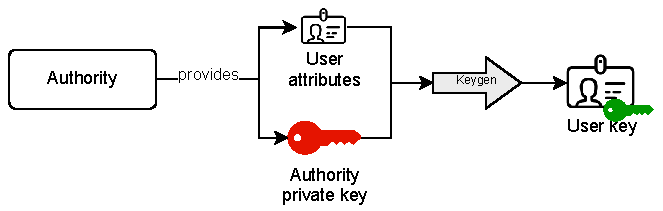
\includegraphics[width=0.5\textwidth]{images/diagrams/keygen_diagram.pdf} % Make sure this path is correct
            \caption{Authority-based key generation process.}
            \label{fig:keygen_diagram}
        \end{figure}

        \begin{algorithm}[h]
            \caption{Setup Authority.}
            \label{alg:setup_authority}
            \begin{algorithmic}[1]
            \Procedure{SetupAuthority}{authority}
                \State $pk, sk \gets \textsc{generateAuthorityKeys}()$
                \State $\textsc{storeAuthorityKeys}(authority, pk, sk)$
            \EndProcedure
            \end{algorithmic}
        \end{algorithm}

        \begin{algorithm}[h]
            \caption{Key Generation.}
            \label{alg:keygen}
            \begin{algorithmic}[1]
            \Procedure{Keygen}{authority, attribute, user}
                \State $sk \gets \textsc{retrieveAuthorityPrivateKey}(authority)$
                \State $K \gets \textsc{generateKey}(sk, attribute)$
                \State $\textsc{storeKey}(user, K)$
            \EndProcedure
            \end{algorithmic}
        \end{algorithm}

    \section{Access policy and Hybrid Encryption Process}
        \label{sec:hybrid_encryption}

        This section outlines the procedure for securing hIoT data using the hybrid cryptographic workflow, visualized in Figure~\ref{fig:encryption_diagram}. The logic for this procedure is presented in Algorithm~\ref{alg:encryption_process}. The algorithm takes a payload and an access policy as input. It first generates a random symmetric key, $K_{G_T}$, which is an element of the pairing group $G_T$. This key is then used to create a hashed AES key, $K_{\textsc{SHA}}$. The output is a two-part ciphertext, consisting of the MA-ABE-encrypted symmetric key, $E_{K_{G_T}}$, and the AES-encrypted payload, $E_{\text{payload}}$. The MA-ABE encryption procedure uses the public keys, $K_A$, of the authorities, $A$, involved, which are retrieved based on the specified access policy. 

        The access policy is defined as a boolean expression over user attributes, allowing for complex conditions on who can access the data. For example, a policy might specify that only users with the attributes 'doctor' at 'HOSPITAL' and 'researcher' at 'UNIVERSITY' can access the data, or alternatively, users with the attribute 'regulator' at 'GOVERNMENT'. The format for such a policy is shown in Equation~\ref{eq:policy_example}.

        \begin{multline}
            \label{eq:policy_example}
            \texttt{doctor@HOSPITAL AND researcher@UNIVERSITY}\\
            \texttt{OR regulator@GOVERNMENT}
        \end{multline}

        \begin{figure}[h]
            \centering
            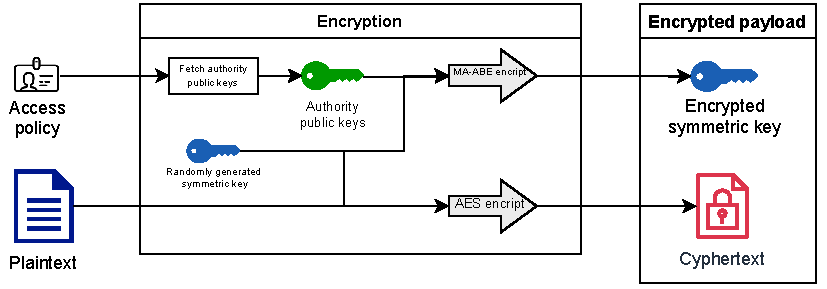
\includegraphics[width=\textwidth]{images/diagrams/encryption_diagram.pdf} % Make sure this path is correct
            \caption{The hybrid encryption process combining MA-ABE and AES.}
            \label{fig:encryption_diagram}
        \end{figure}

        \begin{algorithm}[h]
            \caption{Encryption Process.}
            \label{alg:encryption_process}
            \begin{algorithmic}[1]
            \Procedure{Encrypt}{payload, policy}
                \State $K_{G_T} \gets \textsc{Random}(G_T)$
                \State $A \gets \textsc{getAuthorities}(\text{policy})$
                \State $K_{\textsc{A}} \gets \textsc{retrievePublicKeys}(A)$
                \State $K_{\textsc{SHA}} \gets \textsc{SHA256}(K_{G_T})$
                \State $E_{K_{G_T}} \gets \textsc{maabe.Encrypt}(K_{\textsc{A}}, K_{G_T}, \text{policy})$
                \State $E_{\text{payload}} \gets \textsc{AES.encrypt}(\text{payload}, K_{\textsc{SHA}})$
                \State \Return $E_{K_{G_T}}, E_{\text{payload}}$
            \EndProcedure
            \end{algorithmic}
        \end{algorithm}

    \section{Decryption Process}
        \label{sec:policy_decryption}

        This section details how authorized users recover plaintext data. Access is governed by policies, as defined in Section~\ref{sec:hybrid_encryption}. To recover the data, a user must possess a set of attribute keys that satisfies the encryption policy. The decryption workflow, illustrated in Figure~\ref{fig:decryption_diagram}, shows that the user first decrypts the MA-ABE-encrypted symmetric key and then uses that key to decrypt the data payload. This enforces the access policy. 

        Algorithm~\ref{alg:decryption_process} details the decryption process. It takes three inputs: the MA-ABE-encrypted symmetric key, $E_{K_{G_T}}$; the AES-encrypted payload, $E_{\text{payload}}$; and the user's set of attribute keys, $K_{\text{user}}$. It begins by using the user's attribute keys to recover the original symmetric key, $K_{G_T}$ via the function \textsc{maabe.Decrypt}. This recovered symmetric key is then processed to derive the hashed AES key, $K_{\textsc{SHA}}$. Finally, the \textsc{AES.decrypt} function uses $K_{\textsc{SHA}}$ to decrypt $E_{\text{payload}}$, yielding the original plaintext $payload$. The algorithm then returns this recovered $payload$.


        \begin{figure}[h]
            \centering
            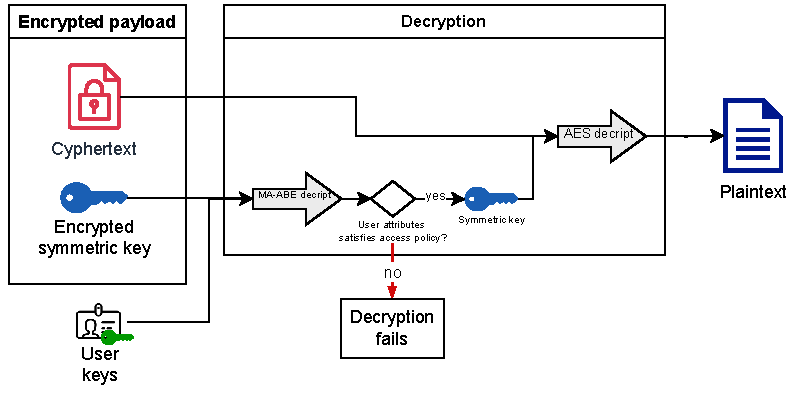
\includegraphics[width=\textwidth]{images/diagrams/decryption_diagram.pdf} % Make sure this path is correct
            \caption{The decryption process for recovering the original data payload.}
            \label{fig:decryption_diagram}
        \end{figure}

        \begin{algorithm}[h]
            \caption{Decryption Process.}
            \label{alg:decryption_process}
            \begin{algorithmic}[1]
            \Procedure{Decrypt}{$E_{K_{G_T}}$, $E_{\text{payload}}$, $K_{\text{user}}$}
                \State $K_{G_T} \gets \textsc{maabe.Decrypt}(E_{K_{G_T}}, K_{\text{user}})$
                \State $K_{\textsc{SHA}} \gets \textsc{SHA256}(K_{G_T})$
                \State $payload \gets \textsc{AES.decrypt}(E_{\text{payload}}, K_{\textsc{SHA}})$
                \State \Return $payload$
            \EndProcedure
            \end{algorithmic}
        \end{algorithm}

    % \section{Hybrid Multi-Authority Attribute-Based Encryption Scheme for Securing HIoT Data}
    %     \label{sec:encryption}

    %     This section presents the cryptographic core of the proposed solution, which uses a hybrid encryption scheme combining MA-ABE and symmetric encryption using AES. The goal is to achieve efficient, fine-grained access control for large hIoT payloads.

    %     \subsection{Overview of the Encryption and Decryption Workflows}
    %         The encryption process consists of the following stages:
    %         \begin{enumerate}
    %             \item Authorities are initialized and generate public/private key pairs.
    %             \item Users are assigned attributes and corresponding secret keys by the authorities.
    %             \item A symmetric key is randomly generated as an element of the pairing group $G_T$.
    %             \item The symmetric key is hashed with SHA-256 to derive an AES key.
    %             \item The payload is encrypted with AES.
    %             \item The original symmetric key is encrypted using MA-ABE under a specified attribute policy.
    %         \end{enumerate}

    %         The decryption process involves the following steps:
    %         \begin{enumerate}
    %             \item Users possess secret keys associated with their attributes, issued by different authorities.
    %             \item The encrypted symmetric key (an element of $G_T$) is decrypted using MA-ABE, if the user's attributes satisfy the access policy.
    %             \item The recovered element from $G_T$ is hashed with SHA-256 to derive the AES key.
    %             \item The payload is decrypted using AES with the derived key.
    %             \item The plaintext is unpadded to retrieve the original data.
    %         \end{enumerate}

    %         This ensures that only users who possess the required attributes can decrypt the MA-ABE-encrypted symmetric key and subsequently access the payload.


    %     \subsection{Key Management and Distribution}
    %         The key management system is designed to handle the generation, storage, and distribution of keys securely. Each authority generates its public/private key pair and distributes the public keys to users. The private keys are securely stored and used for generating user-specific keys based on their attributes.

    %     \subsection{Key Generation and Authority Setup}
    %         Authorities generate keys using the MaabeRW15 scheme from the Charm-Crypto library. Each authority is responsible for a disjoint subset of attributes and securely stores its private key. Public keys are distributed system-wide.

    %     \subsection{Access Policy Specification}
    %         Encryption policies are defined using boolean expressions over attributes, such as in the example policy~\ref{eq:policy_example}, where the attributes are specified in the format "<attribute>@<authority>". The policy can include AND, OR, and NOT operations to define complex access conditions. This allows for flexible and fine-grained access control based on user attributes.
    %         This policy structure allows flexible definitions of access, combining multiple authorities and domains.

    %         \begin{equation}
    %             \label{eq:policy_example}
    %             \texttt{(\allowbreak doctor@HOSPITAL \allowbreak AND \allowbreak researcher@UNIVERSITY) \allowbreak OR \allowbreak regulator@GOVERNMENT}
    %         \end{equation}


    %     \subsection{Security and Performance Considerations}
    %         This scheme ensures:
    %         \begin{itemize}
    %         \item \textbf{Fine-grained access control}: via MA-ABE policies.
    %         \item \textbf{Efficiency}: AES handles bulk data, reducing computational cost.
    %         \item \textbf{Scalability}: Multiple authorities reduce centralization and key distribution bottlenecks.
    %         \end{itemize}

    %         Further evaluation of performance and scalability is provided in Chapter~\ref{chap:evaluation}.


\chapter{Experimental Setup}
\label{chap:experimentalsetup}

    This chapter describes the experimental setup used to evaluate the proposed cryptographic system for HIoT data management. It outlines the evaluation strategy, testbed environment, and the tools employed for testing.

    The chapter is structured as follows: Section~\ref{sec:evaluation-strategy} presents the overall implementation and evaluation strategy and its objectives. Section~\ref{sec:testbed} details the testbed environment, including hardware and software specifications, and the various implementation tools utilized.

    \section{Evaluation Strategy}
        \label{sec:evaluation-strategy}
        The primary objectives of the evaluation are to measure the system's performance in terms of response time, determine its scalability under increasing workloads, and assess the cryptographic overhead introduced by the MA-ABE scheme. In addition, we aim to understand how the number of user attributes affects key size and to verify the security of the implementation.

        For this purpose, we implemented an Application Programming Interface (API) based on the Representational State Transfer (REST) architectural style, which provides endpoints for all the operations defined in Chapter~\ref{chap:proposedsolution}. The API was chosen for its simplicity and ease of integration with existing systems, allowing us to focus on the cryptographic aspects without the overhead of a more complex user interface or a full-fledged application. The source code for the API is available on Zenodo~\citep{maabeflask}.

        On top of the API, we used Locust, a Python-based load testing tool, to simulate concurrent users and measure the system's response times under various conditions. The tests were designed to evaluate both the encryption and decryption processes, as well as the overall throughput of the system.

    \section{Testbed Environment}
        \label{sec:testbed}
        This section describes the testbed environment, including the hardware and software configurations, and the specific tools used for implementation and testing.

        \subsection{Hardware and Software Specifications}
        \label{subsec:hardware-software}
            The experiments were conducted on a single machine whose specifications are listed in Table~\ref{tab:machine_specs}. This section describes the hardware and operating system used, providing context for interpreting the performance results presented later in this chapter.

            \begin{table}[h]
                \centering
                \begin{tabular}{|l|l|}
                \hline
                \textbf{Component} & \textbf{Details} \\ \hline
                Operating System & Linux Mint 22.1 (x86\_64) \\ \hline
                Kernel Version & 6.8.0-57-generic \\ \hline
                Processor & AMD Ryzen 5 PRO 7640HS @ 5.015 GHz \\ \hline
                Architecture & x86\_64 (12 threads, 6 physical cores) \\ \hline
                Memory & 14 GiB RAM, 15 GiB swap \\ \hline
                Storage & NVMe SSD \\ \hline
                Python Version & 3.10.17 \\ \hline
                Containerization & Docker 28.0.4, Docker Compose v2.34.0 \\ \hline
                \end{tabular}
                \caption{Machine specifications and environment configuration used in testing.}
                \label{tab:machine_specs}
            \end{table}

        \subsection{Implementation and Testing Tools}
        \label{subsec:tools}

            To evaluate the implementation of the proposed scheme, we utilized several tools and frameworks that support API development, cryptographic computation, concurrency management, and load testing.

            \textbf{Locust} is a Python-based API load testing tool that allows the definition of user behavior scenarios to simulate concurrent usage. It generates load on the system to evaluate responsiveness and performance under various conditions. We configured it with varying numbers of users and spawn rates to assess scalability.

            \textbf{Gunicorn} is a Web Server Gateway Interface (WSGI) server for Python applications. It enables concurrent request handling through configurable worker processes and threads. We varied the number of threads and workers to test different concurrency configurations and identify an optimal setup.

            \textbf{Charm-Crypto} is a Python library for pairing-based cryptography that offers high-level abstractions for implementing complex cryptographic protocols. It supports a variety of schemes, including MA-ABE. In our implementation, we used the \emph{MaabeRW15} scheme proposed by Rouselakis and Waters~\citep{rouselakis2015efficient}, which provides efficient support for multi-authority setups. Charm-Crypto handled all cryptographic operations in our system.

            \textbf{Flask} is a lightweight web framework for Python used to implement the RESTful API for encryption and decryption operations. Its simplicity and extensibility made it suitable for rapid prototyping of the service layer.

            \textbf{Flask-RESTX} is an extension to Flask that provides tooling for building REST APIs, including automatic request parsing and Swagger documentation support. It was used to define and document the API endpoints in a structured and maintainable way.

            \textbf{Redis} is an in-memory key-value store used for managing and persisting cryptographic keys across authorities and users. In our implementation, Redis served as a lightweight and fast-access backend for storing public/private key pairs and attribute-based user keys during testing. It was deployed as a service within a Docker Compose network, alongside the API, ensuring isolated environments and consistent behavior across test executions.

            All services, including the API, Redis, and test agents, were containerized using Docker and orchestrated with Docker Compose to enable reproducible testing conditions and simplify deployment.

\chapter{Evaluation}
    \label{chap:evaluation}
    This chapter presents the implementation details and performance evaluation of the cryptographic system proposed in the previous chapters. We describe the technologies used, the deployment environment, the testing methodology, and the results obtained under different configurations. To ensure reproducibility of results, all source code developed for this project has been archived and made publicly available through Zenodo~\citep{maabeflask}.

    

    

        % Deprecated section. The results are not relevant anymore.
        % \subsection{Failure Rate}
        %     \label{sec:failurerate}
        %     This test was done with the Locust framework to determine the failure rate of the system. The test was conducted with a payload size of 1KB and 1000 users. The failure rate was calculated by the number of failed requests divided by the total number of requests.

        %     The locustfile used for the test defines 80\% of the users as clients and 20\% as authorities. Each authority instance calls the endpoint \emph{/api/setup\_authority} once upon instantiation, and subsequently calls \emph{/api/keygen} for a user following a Round-Robin strategy. The client instances call the \emph{/api/encrypt} endpoint with a random payload and access policy and then call the \emph{/api/decrypt} endpoint with the encrypted payload and the user's key with a 50\% probability of calling each endpoint.
            
        %     The test was run for 15 minutes with a spawn rate of 100 user per second. The failure rate was calculated as the number of failed requests divided by the total number of requests.

        %     \begin{figure}[h]
        %         \centering
        %         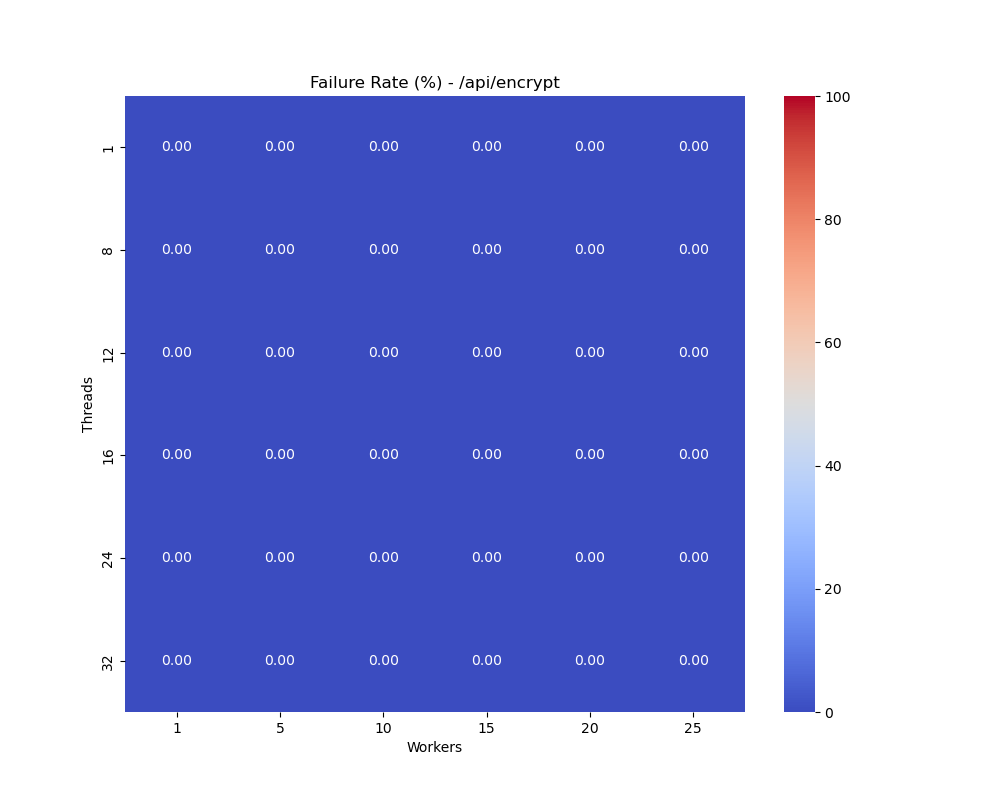
\includegraphics[width=\textwidth]{images/phase1/failure_rate__api_encrypt.png}
        %         \caption{Failure rate for /api/encrypt for different configurations of threads and workers}
        %         \label{fig:failurerateencrypt}
        %     \end{figure}

        %     \begin{figure}[h]
        %         \centering
        %         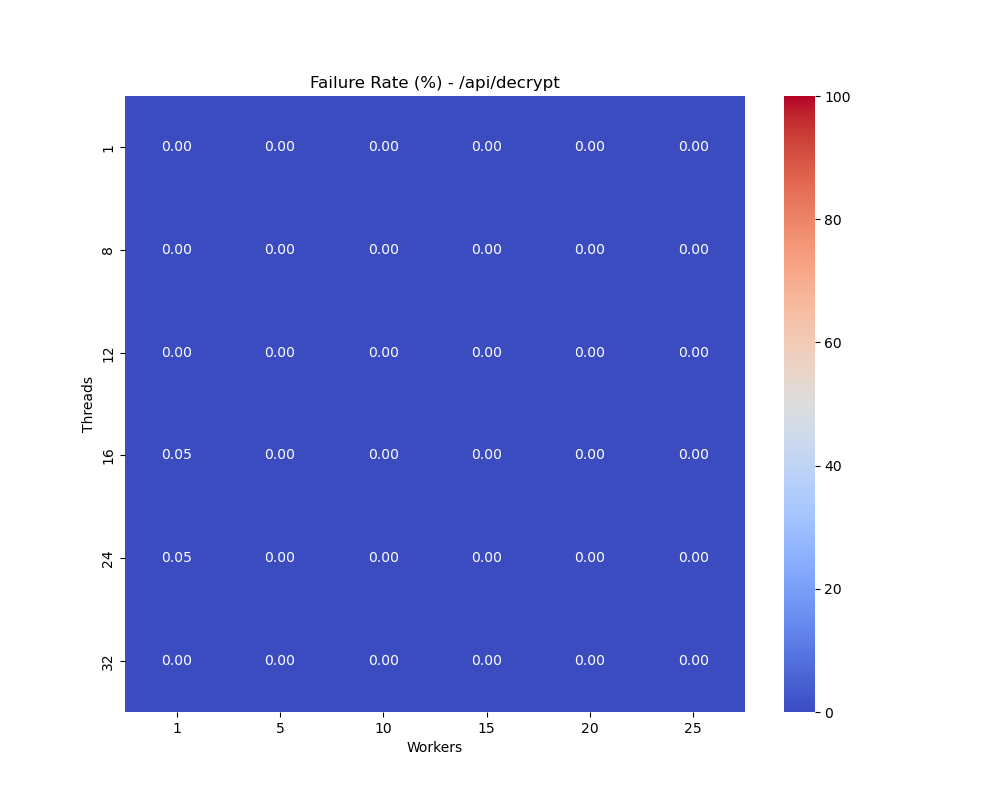
\includegraphics[width=\textwidth]{images/phase1/failure_rate__api_decrypt.png}
        %         \caption{Failure rate for /api/decrypt for different configurations of threads and workers}
        %         \label{fig:failureratedecrypt}
        %     \end{figure}


        \section{Concurrency analysis}
        \label{subsec:phase1_concurrency}

        The first phase of our analysis aimed to determine the optimal configuration of Gunicorn workers and threads for concurrent request handling. We fixed the payload size at 1\,KB, the number of concurrent users at 100, and the number of attributes in the encryption policy at one. The number of threads and workers was varied according to Formula~\ref{form:numberthreadsworkers}.

        \begin{equation}
            \label{form:numberthreadsworkers}
            (\text{threads}, \text{workers}) \mid \text{threads} \in \{1, 8, 12, 16, 24, 32\}, \text{workers} \in \{1, 5, 10, 15, 20, 25\} 
        \end{equation}

        Figure~\ref{fig:encrypt_response_time_workers} and Figure~\ref{fig:decrypt_response_time_workers} shows the response time for encryption and decryption with a fixed number of workers while varying the number of threads. The results indicate a relatively stable median response time across thread counts, suggesting that the system does not benefit significantly from thread-level concurrency.

        Figure~\ref{fig:encrypt_response_time_threads} and Figure~\ref{fig:decrypt_response_time_threads}, in contrast, presents the effect of increasing the number of workers with a fixed thread count. The response time decreases exponentialy as more workers are added, showing that the system benefits from process-based concurrency.

        Based on these results, we adopted a configuration of 25 workers and 1 thread for the remaining test phases. This choice aligns with Gunicorn's recommendation\footnote{\url{https://docs.gunicorn.org/en/latest/design.html\#how-many-workers}} for the optimal number of workers, given by Equation~\ref{form:numberworkers}, where \texttt{cores} is the number of logical cores available. The request times for this configuration can be seen in Table~\ref{tab:response_times}.

        \begin{equation}
            \label{form:numberworkers}
            \text{workers} = (2 \times \text{cores}) + 1
        \end{equation}

        \begin{figure}
            \centering
            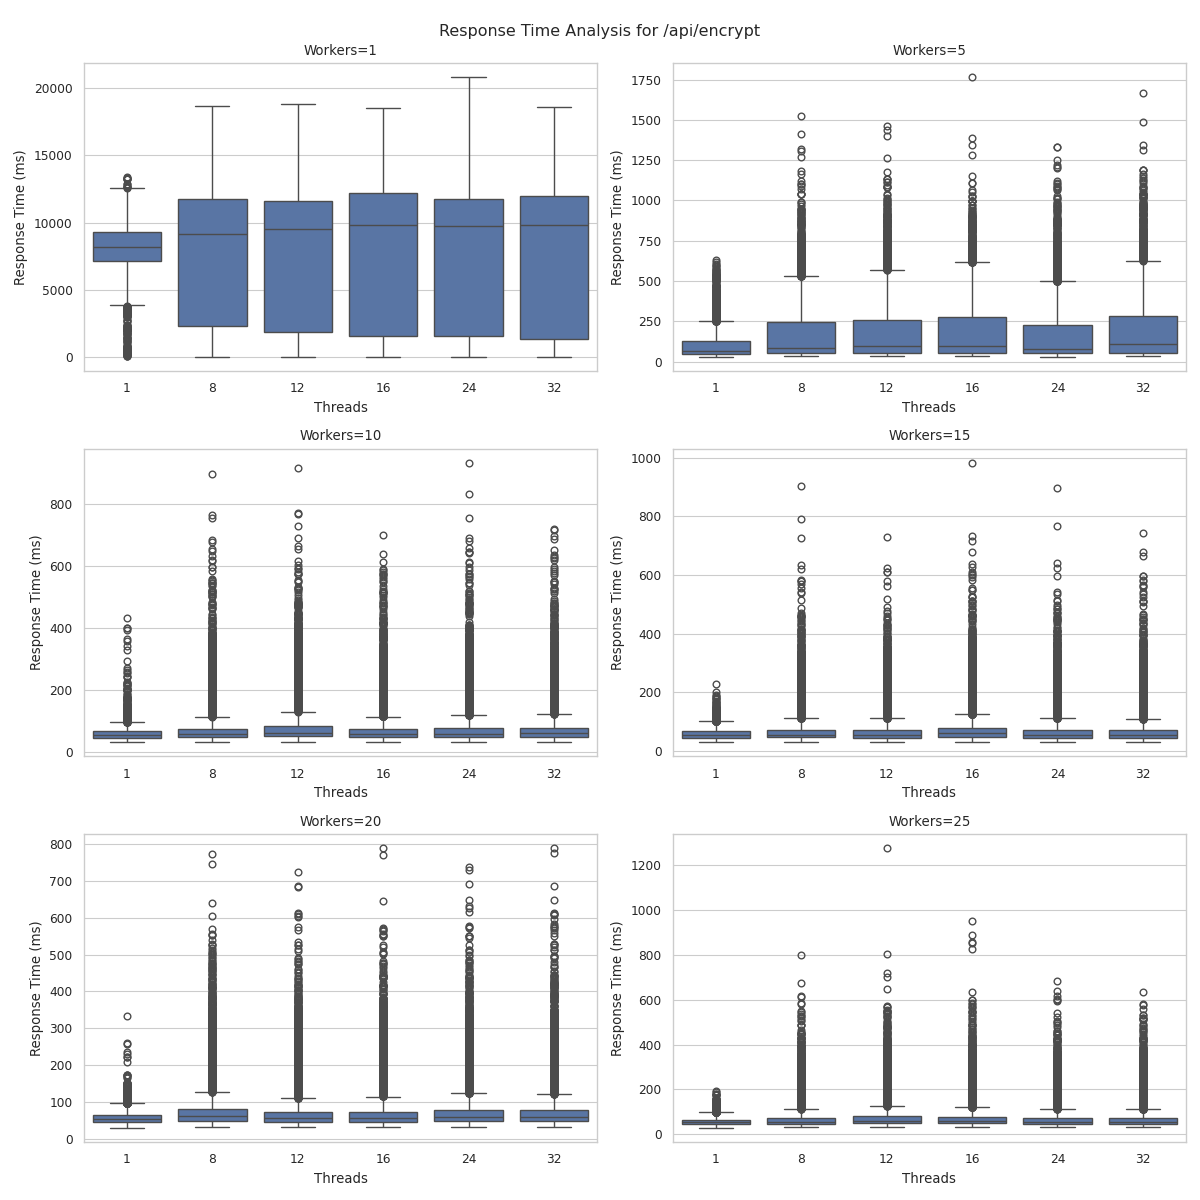
\includegraphics[width=\textwidth]{images/phase1/api_encrypt/response_time_workers_summary.png}
            \caption{Encryption response time varying the number of threads (workers fixed).}
            \label{fig:encrypt_response_time_workers}
        \end{figure}

        \begin{figure}
            \centering
            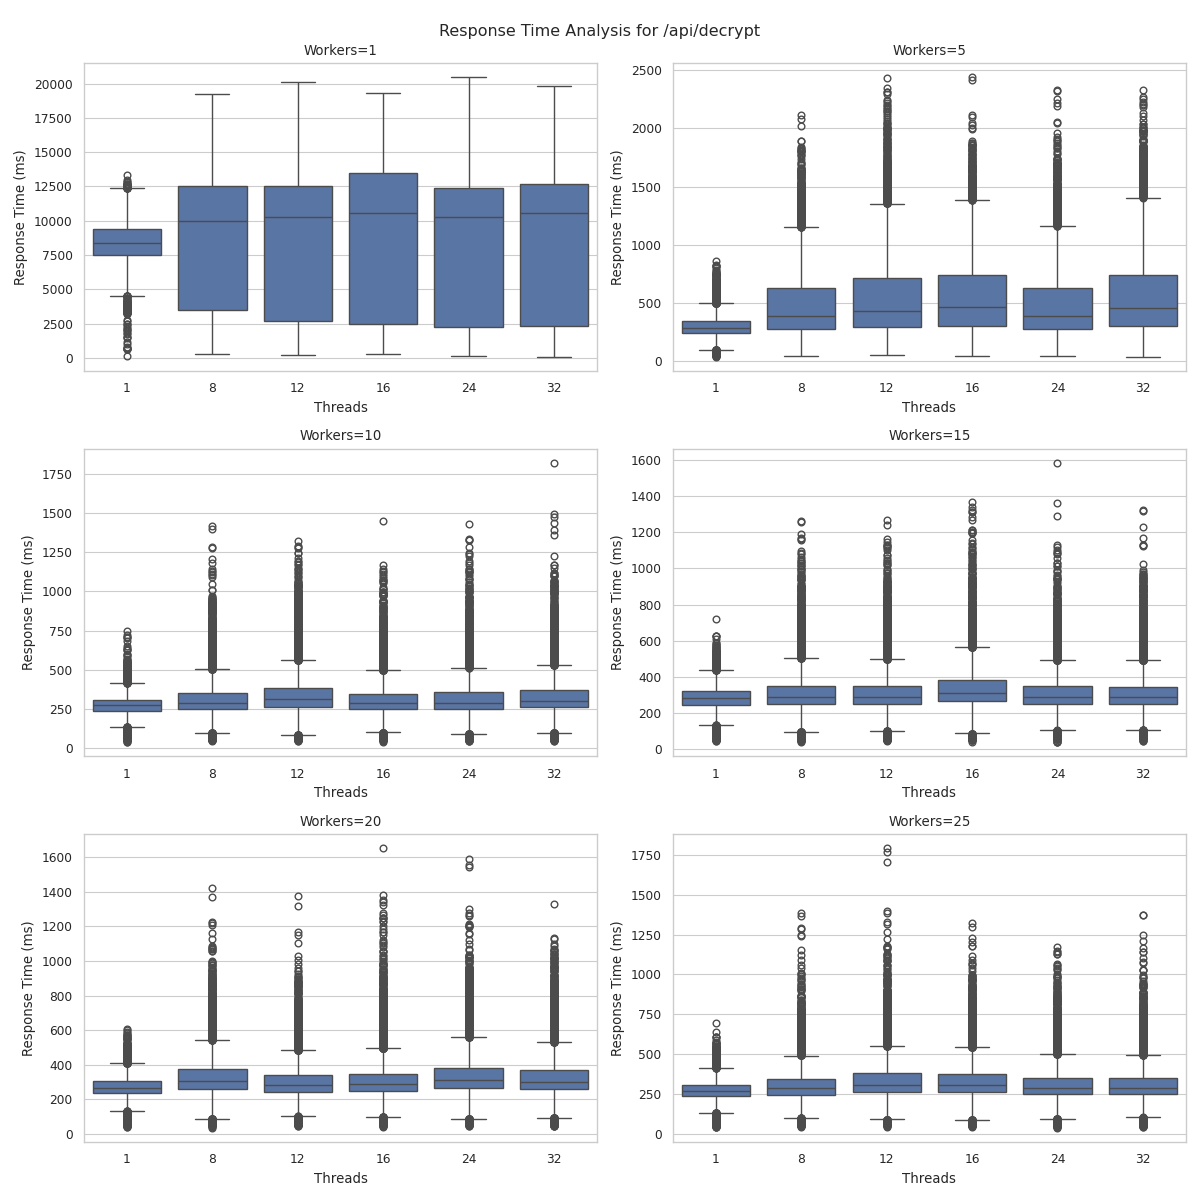
\includegraphics[width=\textwidth]{images/phase1/api_decrypt/response_time_workers_summary.png}
            \caption{Decryption response time varying the number of threads (workers fixed).}
            \label{fig:decrypt_response_time_workers}
        \end{figure}

        \begin{figure}
            \centering
            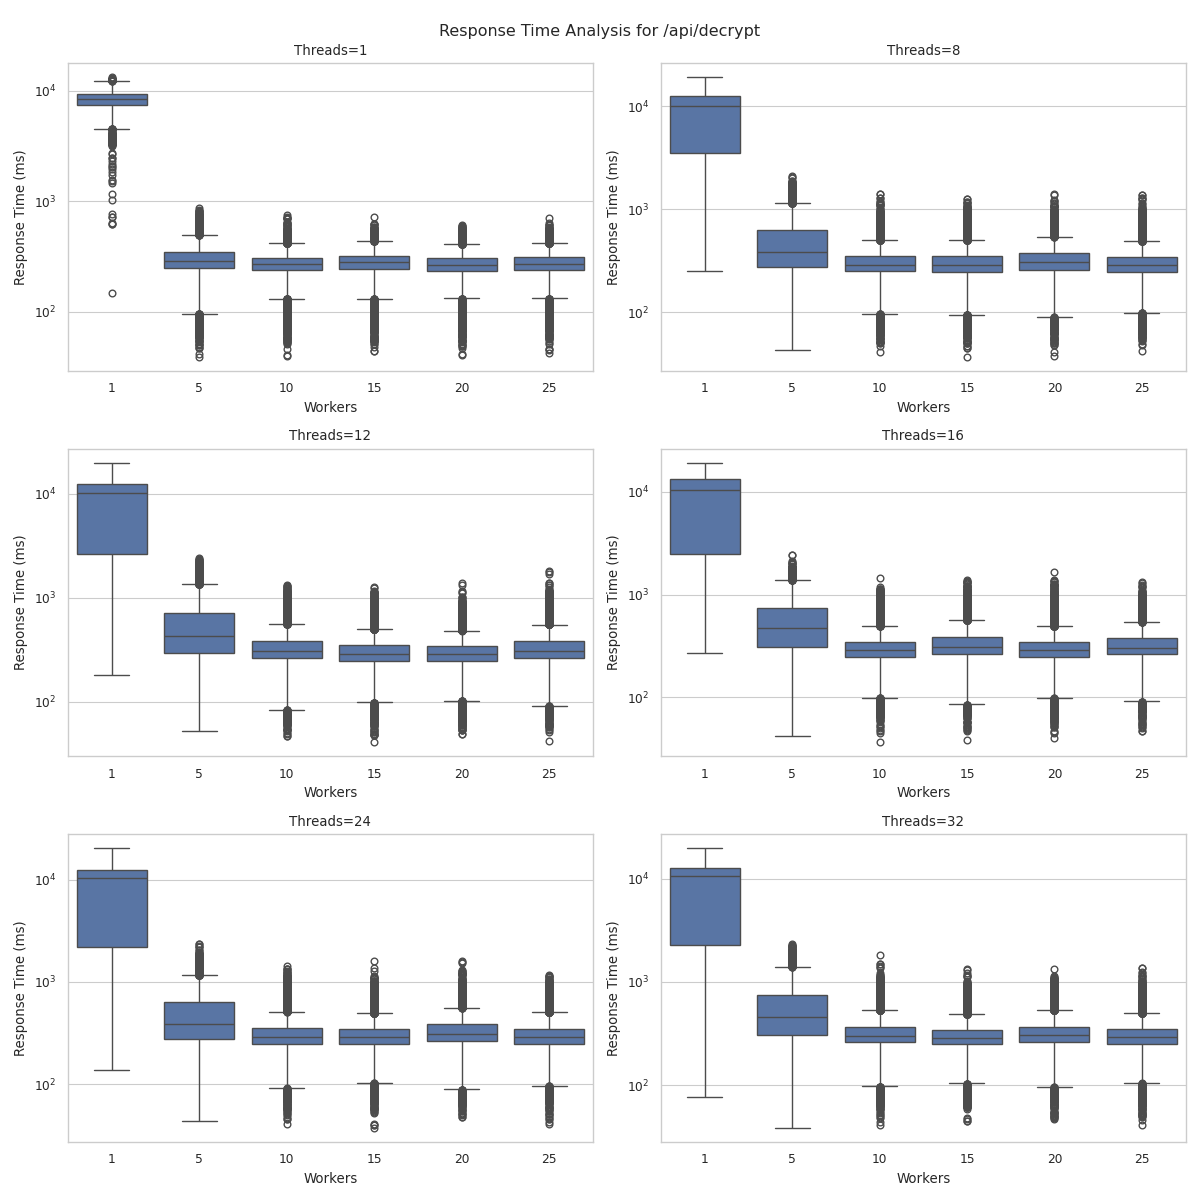
\includegraphics[width=\textwidth]{images/phase1/api_decrypt/response_time_threads_summary.png}
            \caption{Encryption response time varying the number of workers (threads fixed).}
            \label{fig:encrypt_response_time_threads}
        \end{figure}

        \begin{table}
                \centering
                \begin{tabular}{|l|l|l|l|l|}
                \hline
                    Endpoint & Mean Response Time (ms) & Std Dev (ms) & Total Requests & RPS \\ \hline
                    /api/decrypt & 273.51 & 71.38 & 7423 & 12.45 \\ \hline
                    /api/encrypt & 57.37 & 52.18 & 7539 & 12.59 \\ \hline
                \end{tabular}
                \caption{Summary of response times for encryption and decryption using 25 workers and 1 thread. RPS stands for Requests Per Second.}
                \label{tab:response_times}
            \end{table}

        \begin{figure}
            \centering
            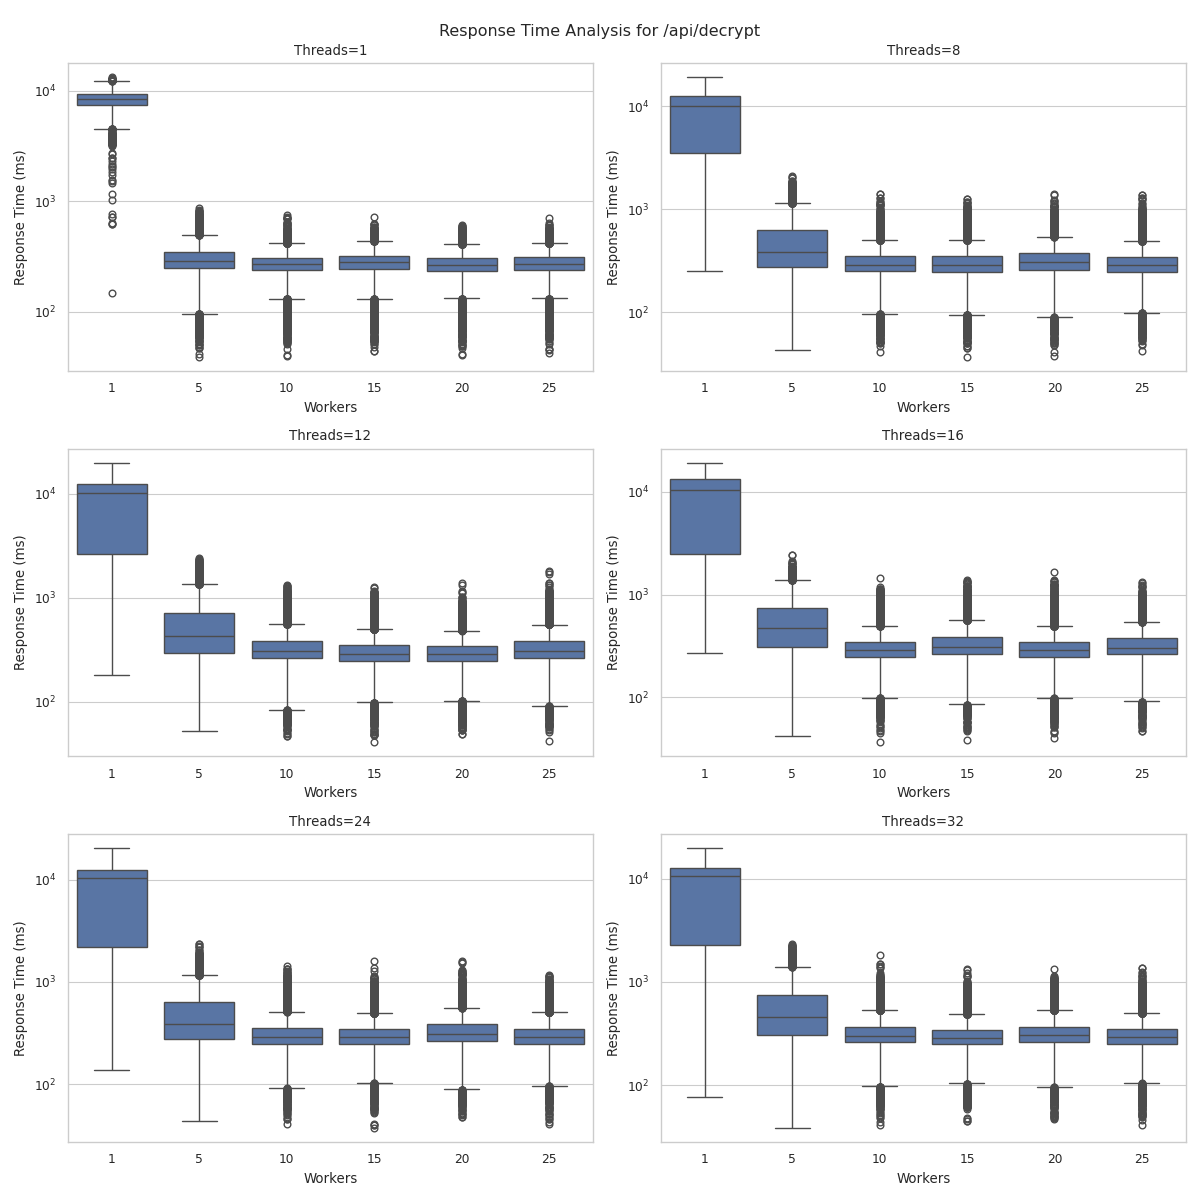
\includegraphics[width=\textwidth]{images/phase1/api_decrypt/response_time_threads_summary.png}
            \caption{Decryption response time varying the number of workers (threads fixed).}
            \label{fig:decrypt_response_time_threads}
        \end{figure}


        \section{Payload Size Impact Analysis}
        \label{subsec:phase2_payload}

            In the second phase, we evaluated the impact of payload size on the system's performance. The number of workers and threads was fixed at 25 and 1, respectively, and the number of users was kept at 100. The payload size was varied according to Formula~\ref{form:payloadsizes}.

            \begin{equation}
            \label{form:payloadsizes}
                \text{payload\_size} \in \{1\text{KB}, 4\text{KB}, 16\text{KB}, 32\text{KB}, 64\text{KB}, 256\text{KB}\}
            \end{equation}

            Figures~\ref{fig:encrypt_payload_size} and~\ref{fig:decrypt_payload_size} present the encryption and decryption response times, respectively, for different payload sizes. As expected, response time increases with larger payloads. However, the encryption process shows a more gradual increase compared to decryption, which may reflect higher complexity in the MA-ABE decryption routine. Table~\ref{tab:response_times} summarizes the mean response times and standard deviations for both encryption and decryption operations across all payload sizes. An original payload of 32KB expands to approximately 87KB, and a 256KB payload increases to about 699KB after encryption. This substantial expansion directly affects the storage requirements and bandwidth utilization for data retrieval from IPFS, especially crucial in resource-constrained hIoT environments where storage efficiency and network overhead are critical considerations. 
            

            \begin{figure}
                \centering
                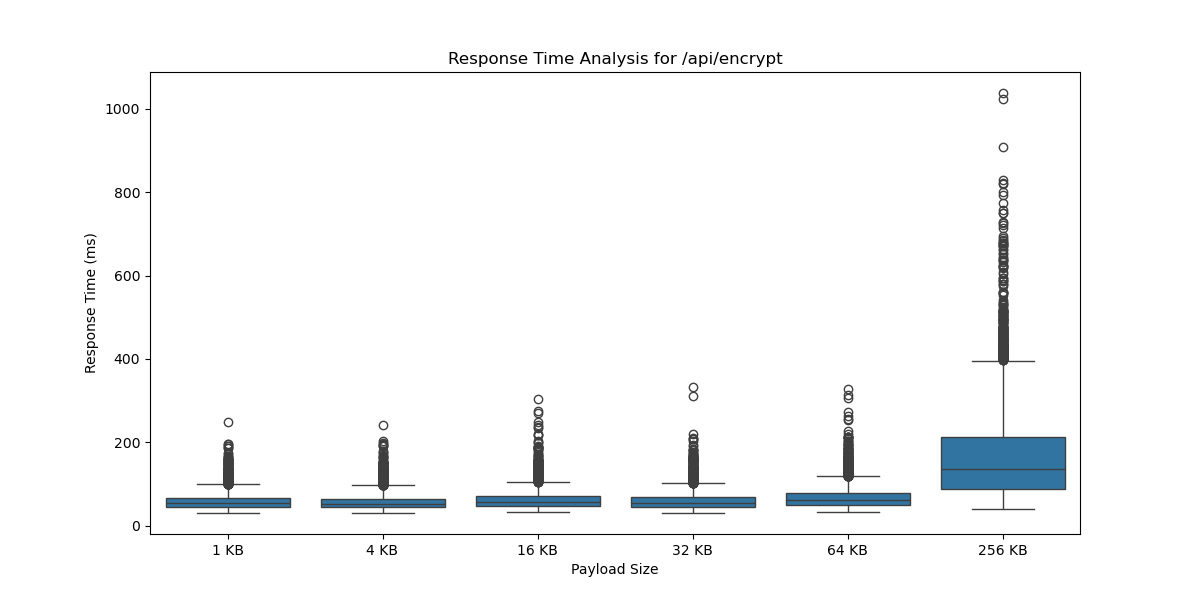
\includegraphics[width=\textwidth]{images/phase2/response_time_api_encrypt.png}
                \caption{Encryption response time for different payload sizes.}
                \label{fig:encrypt_payload_size}
            \end{figure}

            \begin{figure}
                \centering
                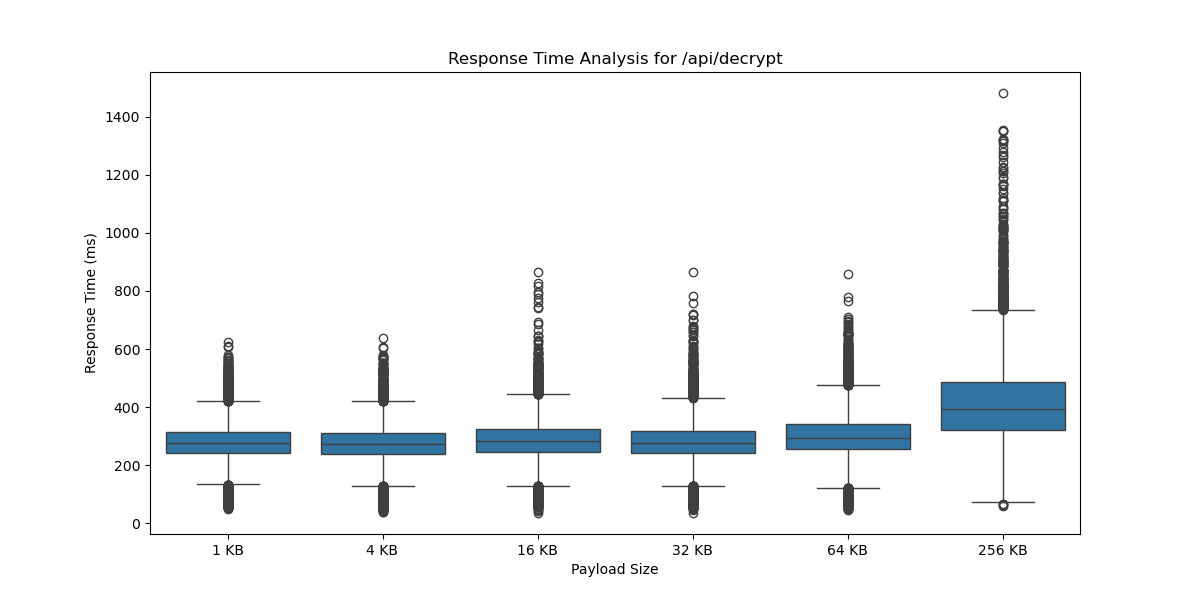
\includegraphics[width=\textwidth]{images/phase2/response_time_api_decrypt.png}
                \caption{Decryption response time for different payload sizes.}
                \label{fig:decrypt_payload_size}
            \end{figure}

        \section{User Load Analysis}
        \label{subsec:user_load_analysis}

            To examine how the system scales with increasing numbers of concurrent users, we varied the number of users according to Formula~\ref{form:userload}. The payload size was fixed at 64\,KB (chosen based on the payload size analysis), and the number of workers and threads remained 25 and 1, respectively.

            \begin{equation}
            \label{form:userload}
                \text{users} \in \{10, 50, 100, 250, 500, 1000\}
            \end{equation}

            Figures~\ref{fig:encrypt_user_load} and~\ref{fig:decrypt_user_load} illustrate the effect of user load on response time. As expected, response time increases as more users are introduced. The system handles moderate user loads well, but performance degradation becomes more pronounced at the highest concurrency levels.

            \begin{figure}
                \centering
                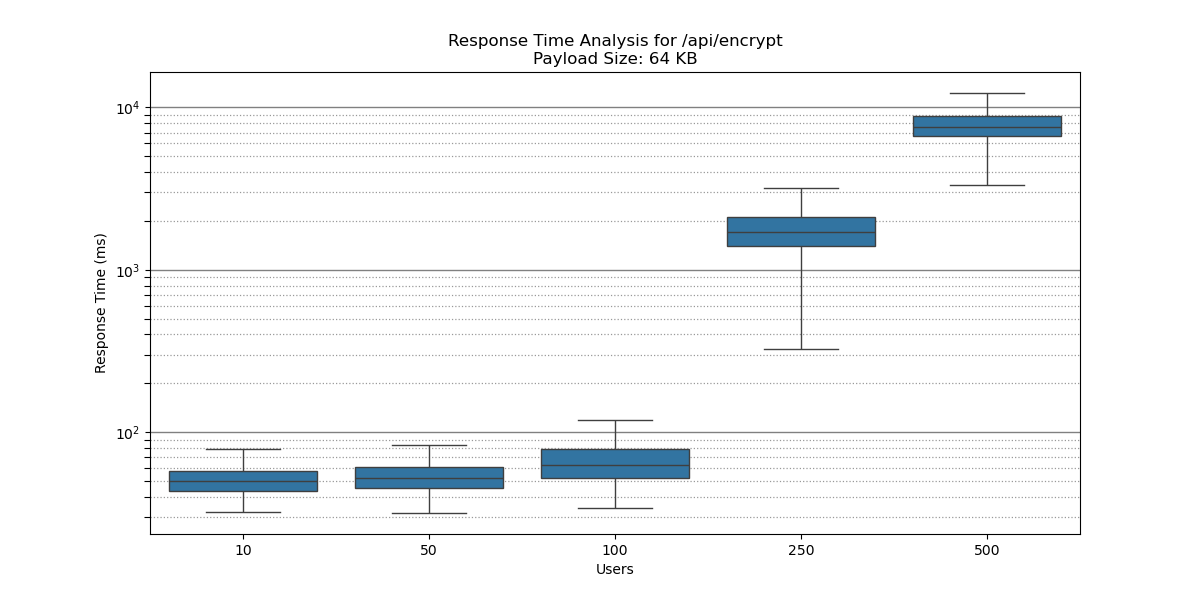
\includegraphics[width=\textwidth]{images/phase3/response_time_api_encrypt_64KB.png}
                \caption{Encryption response time for different user loads.}
                \label{fig:encrypt_user_load}
            \end{figure}

            \begin{figure}
                \centering
                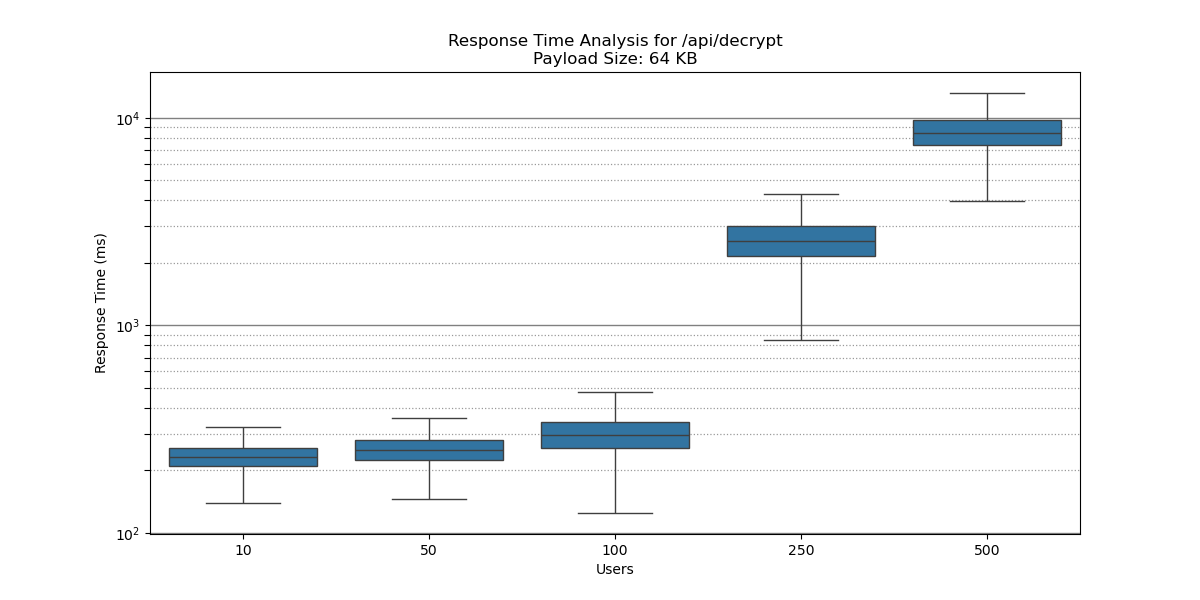
\includegraphics[width=\textwidth]{images/phase3/response_time_api_decrypt_64KB.png}
                \caption{Decryption response time for different user loads.}
                \label{fig:decrypt_user_load}
            \end{figure}

        \section{Encryption Policy Size Analysis}
        \label{subsec:encryption_policy_size_analysis}

            To assess how the size of the encryption policy affects performance, we varied the number of attributes in the access policy from 1 to 10. The other parameters (payload size = 64\,KB, users = 100, workers = 25, threads = 1) were kept fixed.

            Figures~\ref{fig:encrypt_policy_size} and~\ref{fig:decrypt_policy_size} show how increasing the number of attributes in the policy affects encryption and decryption times. As expected, more complex policies result in higher response times due to the additional computational overhead involved in evaluating attribute trees and pairing operations.

            \begin{figure}
                \centering
                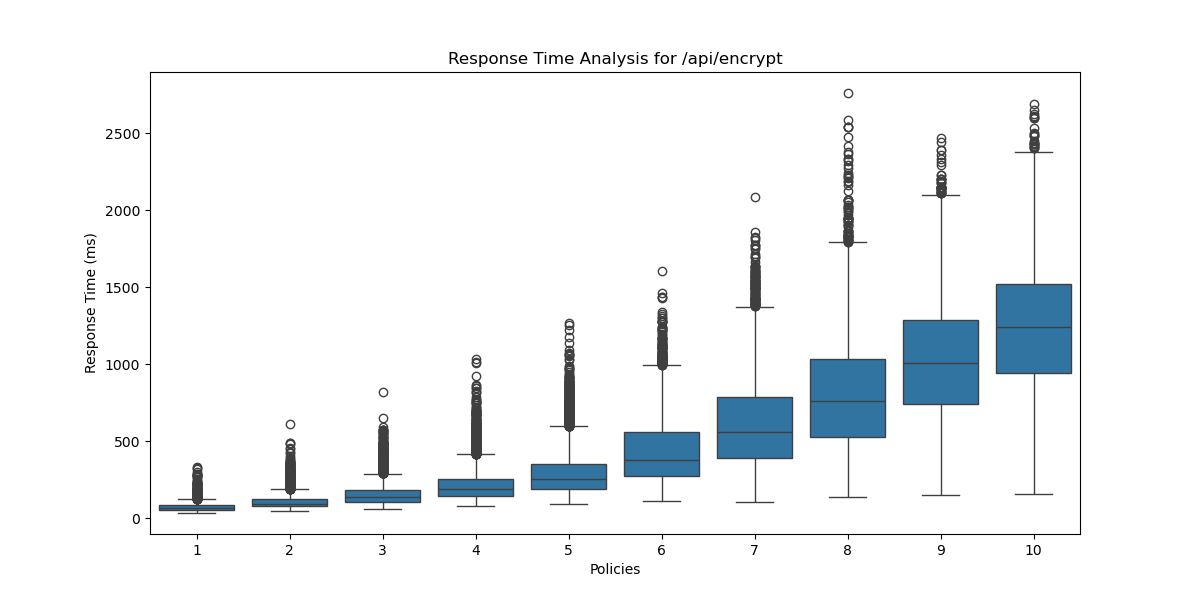
\includegraphics[width=\textwidth]{images/phase4/response_time_api_encrypt.png}
                \caption{Encryption response time for different policy sizes.}
                \label{fig:encrypt_policy_size}
            \end{figure}

            \begin{figure}
                \centering
                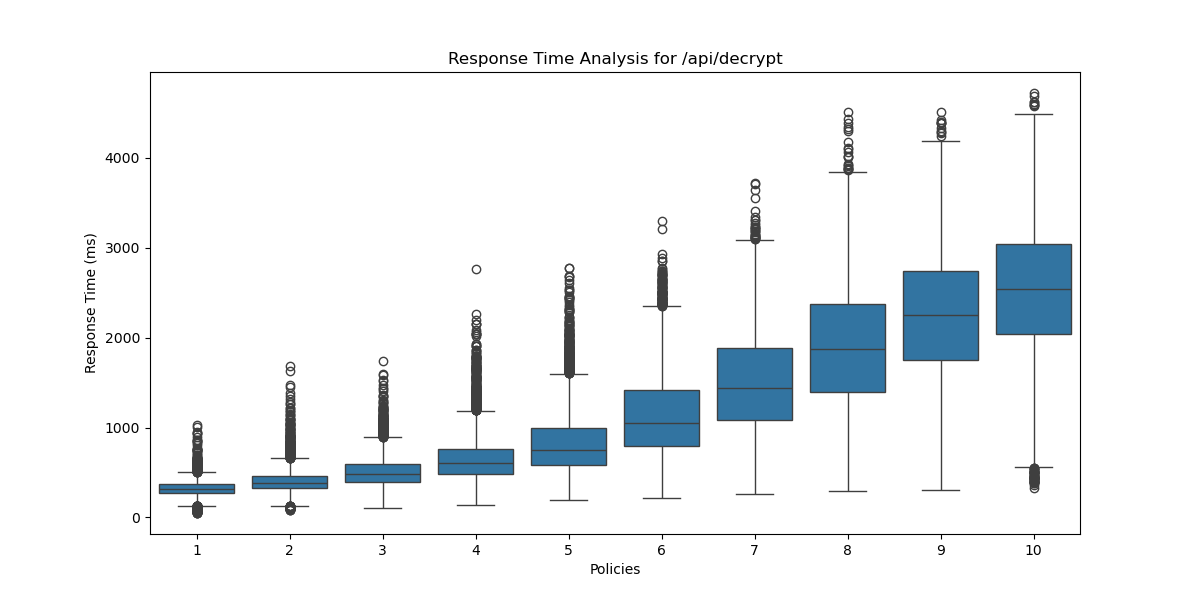
\includegraphics[width=\textwidth]{images/phase4/response_time_api_decrypt.png}
                \caption{Decryption response time for different policy sizes.}
                \label{fig:decrypt_policy_size}
            \end{figure}

        
        \section{User key size}
            \label{sec:keysize}
            Figure~\ref{fig:user_key_size} shows the size of the user key for different number of attributes. The user key size increases linearly, reaching 25KB for 100 attributes.

            The evaluation of user key size reveals a linear correlation with the number of attributes assigned to a user, as illustrated in Figure~\ref{fig:user_key_size}. For instance, a user key can reach approximately 25KB for 100 attributes. This characteristic has significant implications for the overall storage footprint within IPFS architecture proposed by \citet{laura2023}. In her framework, data payloads are stored in IPFS blocks, and while our cryptographic scheme primarily encrypts the symmetric key rather than the entire payload with MA-ABE, the original payload itself also undergoes encryption with AES, and is then coupled with the encrypted symmetric key. This process introduces a measurable overhead to the size of the data being stored on IPFS. This highlights a fundamental trade-off, common to all cryptographic systems.

            \begin{figure}
                \centering
                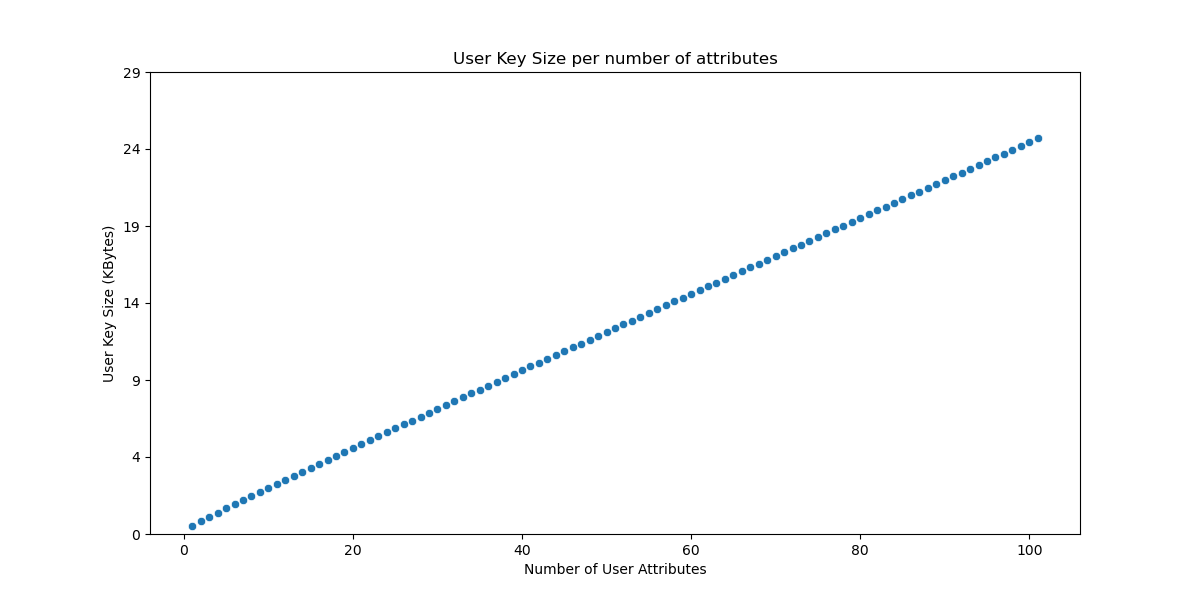
\includegraphics[width=\textwidth]{images/key_size_analysis/user_key_size_analysis.png}
                \caption{Comparison of user key size for different number of attributes.}
                \label{fig:user_key_size}
            \end{figure}


        \section{Discussion}
            \label{sec:discussion}
            The performance evaluation presented in this chapter provides critical insights into the feasibility and operational trade-offs of the proposed hybrid MA-ABE scheme. The results from the concurrency, payload size, user load, and policy complexity analyses collectively inform the practical application of this cryptographic layer within an HIoT framework, such as the one proposed by \citet{laura2023}.

            \subsection{Interpreting Performance and Scalability}

                Our analysis of Gunicorn worker configurations (Section~\ref{subsec:phase1_concurrency}) revealed that system performance scales effectively with the number of processes (workers) but does not benefit from multi-threading. As shown in Figures~\ref{fig:encrypt_response_time_threads} and~\ref{fig:decrypt_response_time_threads}, increasing the number of workers leads to a significant decrease in response times. Conversely, increasing the number of threads per worker offered no discernible performance improvement (Figures~\ref{fig:encrypt_response_time_workers} and~\ref{fig:decrypt_response_time_workers}). This behavior is characteristic of CPU-bound Python applications due to the Global Interpreter Lock (GIL), which prevents multiple native threads from executing Python bytecodes simultaneously. Since cryptographic operations are computationally intensive, the GIL becomes a bottleneck, neutralizing the benefits of threading. The Charm-Crypto library, while built on C components, is still subject to the GIL when its functions are invoked from Python, explaining this observation. This finding suggests that for deployment, scaling should be achieved by increasing the number of worker processes rather than threads.

                The payload size analysis (Section~\ref{subsec:phase2_payload}) demonstrated that while encryption and decryption times increase with payload size, the system remains efficient. For instance, encrypting a 256\,KB payload takes, on average, 165.6 ms, and decryption takes 419.4 ms. The hybrid nature of our scheme, which uses the computationally expensive MA-ABE only to protect a small symmetric key, proves effective. The bulk of the work, encrypting the payload itself, is handled by the highly efficient AES algorithm. This confirms the suitability of the hybrid approach for securing large HIoT data payloads without incurring prohibitive computational costs.

                The user load and policy size analyses highlight important scalability limitations. Decryption time increases substantially with both the number of concurrent users (Section~\ref{subsec:user_load_analysis}) and the number of attributes in the access policy (Section~\ref{subsec:encryption_policy_size_analysis}). The growth in response time with policy complexity (Figure~\ref{fig:decrypt_policy_size}) is expected, as MA-ABE decryption requires a number of pairing operations proportional to the number of attributes in the policy. This underscores a fundamental trade-off between the granularity of access control and system performance. For practical HIoT applications, policies should be designed to be as concise as possible to ensure acceptable latency.

            \subsection{Impact on Decentralized Storage}

                A key consideration for integrating this cryptographic layer into the architecture proposed by \citet{laura2023} is its impact on storage. Our analysis in Section~\ref{sec:keysize} shows that user key size grows linearly with the number of attributes, reaching approximately 25\,KB for 100 attributes. Furthermore, the AES-encrypted payload, combined with the MA-ABE encrypted symmetric key, introduces storage overhead. For example, a 256\,KB payload expands to approximately 699\,KB after encryption.

                In the context of a decentralized storage system like IPFS, this expansion affects not only storage capacity but also network bandwidth, as larger objects must be transferred between peers. This highlights a trade-off: the robust, fine-grained security provided by the scheme comes at the cost of increased storage and network resource consumption, which must be considered when deploying the system in resource-constrained HIoT environments.

            \subsection{Connecting Findings to the Research Problem}

                The evaluation successfully demonstrates that the proposed hybrid MA-ABE scheme provides a concrete and viable solution to the cryptographic gap identified in foundational hIoT architectures like that of \citet{laura2023}. Our implementation addresses the need for fine-grained, multi-stakeholder access control, which is a significant limitation of traditional encryption methods in healthcare environments. While the performance evaluation reveals scalability trade-offs related to policy complexity and user load, it confirms that the scheme is practical for a range of realistic HIoT use cases. The selection of the robust MaabeRW15 scheme~\citep{rouselakis2015efficient} and its successful implementation and testing also address the critical need for practically verified cryptographic solutions, as noted in the problem statement.


\chapter{Conclusion}
    \label{chap:conclusion}

    This thesis addressed the critical need for robust confidentiality and fine-grained access control in decentralized HIoT data management systems. Building upon foundational architectures that leverage IPFS and blockchain, we identified a significant gap: the absence of a concrete cryptographic layer capable of securing data payloads based on dynamic, attribute-based policies in a multi-stakeholder environment. To fill this gap, we proposed, implemented, and evaluated a hybrid cryptographic scheme combining MA-ABE with AES.

    The evaluation of our proof-of-concept implementation yielded key insights into its practical performance. We demonstrated that the hybrid approach is highly efficient for encrypting large data payloads, as the computationally intensive MA-ABE operations are confined to a small symmetric key. Our analysis confirmed that the system's scalability is dependent on process-based concurrency and is sensitive to the complexity of access policies and the number of concurrent users—highlighting a crucial trade-off between security granularity and performance. The findings validate that the proposed scheme is a viable and effective solution for enforcing fine-grained access control in HIoT systems, significantly enhancing data privacy and security.

    \section{Future Work}
    \label{sec:futurework}

        While this thesis successfully demonstrates the feasibility of the proposed scheme, several avenues for future research remain. The most immediate extension of this work would be to fully integrate the cryptographic module into the complete decentralized storage framework proposed by \citet{laura2023} and conduct an end-to-end latency evaluation that captures cryptographic processing alongside IPFS data retrieval and blockchain transaction times. Furthermore, the current evaluation was conducted on a single-node testbed. Future work should deploy the system in a true distributed environment to accurately assess network latency and real-world scalability. A significant enhancement would be to optimize the handling of binary data. The current system operates on text-based JavaScript Object Notation (JSON) payloads, requiring the conversion of binary data, such as medical images, into inefficient string representations (e.g., Base64), which substantially increases HTTP payload size. Future work could implement direct binary data encryption by modifying the API to accept 'multipart/form-data' requests, allowing the AES algorithm to be applied directly to a binary file stream. The response, containing the encrypted payload, would then be delivered as an 'application/octet-stream'. This would eliminate encoding overhead, reduce network bandwidth consumption, and significantly improve system efficiency, especially for HIoT applications managing large binary files. Additionally, performance could be enhanced by exploring alternative key storage mechanisms, such as in-memory caches or secure hardware modules, to reduce the I/O bottlenecks of the current implementation. Finally, subsequent research could implement and compare the performance of other MA-ABE schemes to further optimize the trade-offs between advanced features and operational efficiency.



\bibliographystyle{abntex2-alf}
\bibliography{biblio}

\end{document}
